
%----------------------------------------------------------------------------------------%
% START LaTeX preamble

% define document type, font and paper size
\documentclass[11pt,a4paper]{article}

%----------------------------------------------------------------------------------------%
% IMPORT LaTeX packages

\usepackage{inputenc}
\usepackage[ngerman, english]{babel}
\usepackage{csquotes}
\usepackage{amsmath}
\usepackage{amssymb}
\usepackage{amsfonts}
\usepackage{graphicx}
\usepackage{wrapfig}
\usepackage[margin=1.25in]{geometry}
\usepackage{pdfpages}
\usepackage{listings}
\usepackage{setspace}
\usepackage{systeme}
\usepackage{mdframed}

%----------------------------------------------------------------------------------------%
% SET user defined commands

\newcommand{\mathsym}[1]{{}}
\newcommand{\unicode}[1]{{}}

%----------------------------------------------------------------------------------------%
% IMPORT LaTeX packages to manange bibliography

% MLA, APA, or IEEE? - https://www.overleaf.com/learn/latex/Biblatex_citation_styles
\usepackage[style=apa]{biblatex}
\addbibresource{bibliography.bib}

%----------------------------------------------------------------------------------------%
% DEFINE header values

% define the cover page values
\title
{
    Assessed exercise 02\\
    49th CIDTEC
}
\author
{
    Antonio Osamu Katagiri Tanaka \\
    A01212611
}
\date{\today}

%----------------------------------------------------------------------------------------%
% USER-DEFINED commands

% Keywords command
\providecommand{\keywords}[1]
{
    \\
    \\
    \small
    \textbf{\textit{Keywords:}} #1
}

%----------------------------------------------------------------------------------------%

\begin{document}

%----------------------------------------------------------------------------------------%
% CREATE the 1st page (cover page)

\maketitle

%----------------------------------------------------------------------------------------%
% DEFINE the abstract text & keywords

%\begin{abstract}
%    \emph
%    {
%        Lorem ipsum dolor sit amet, consectetur adipiscing elit, sed do eiusmod tempor incididunt ut labore et dolore magna aliqua. Ut enim ad minim veniam, quis nostrud exercitation ullamco laboris nisi ut aliquip ex ea commodo consequat. Duis aute irure dolor in reprehenderit in voluptate velit esse cillum dolore eu fugiat nulla pariatur. Excepteur sint occaecat cupidatat non proident, sunt in culpa qui officia deserunt mollit anim id est laborum.
%    }
%    \keywords{Lorem, ipsum, dolor, sit, amet}
%\end{abstract}

%----------------------------------------------------------------------------------------%
\clearpage

%----------------------------------------------------------------------------------------%
% CREATE a table of contents in a new page

\tableofcontents
\clearpage

%----------------------------------------------------------------------------------------%
% CREATE a list of figures and a list of tables in a new page

%\listoffigures
\listoftables
\clearpage

%----------------------------------------------------------------------------------------%
% DOCUMENT body starts here
\section{Overview}\label{sec:overview}
The ``\emph{Congreso de Investigación y Desarrollo}" of \emph{Tecnológico de Monterrey} is evolving towards a new investigation model to match the goals set by the National Schools, the Strategic Approach Research Groups, and the Research Professor Model.

\emph{Tecnológico de Monterrey} has a commitment to research, which constitutes an institutional priority whose objective is to: a) contribute significantly to the academic quality of the teaching-learning process; b) convert scientific and technological knowledge into innovative solutions that benefit society; and c) Transform, through the generation and transfer of knowledge, to the communities in the economic, political and social matters.

The ``\emph{Congreso de Investigación y Desarrollo}" provided the means to present the research developed by teachers and students in the following subjects:

\begin{itemize}
	\item{Public politics}
	\item{Education, Humanities and Social Sciences}
	\item{Medicine}
	\item{Mechatronics}
	\item{Biotechnology}
	\item{Information Technology, Electronics and Communications}
	\item{Sustainable technologies}
	\item{Business}
\end{itemize}

On the other hand, ``\emph{Congreso de Investigación y Desarrollo}" allowed professors, executives, researchers, master's, professional and preparatory students to actively participate in several events such as:

\begin{itemize}
	\item{Conferences/lectures}
	\item{Panels}
	\item{\emph{Rómulo Garza} 2018 Awards}
	\item{Project Presentations}
	\item{Focus-Groups Parallel-Sessions}
	\item{Talks}
	\item{Networking}
	\item{Instructor-Student Workshops}
\end{itemize}

\emph{Tecnológico de Monterrey} outstanding leaders participated in the event within the research areas which have been identified as \emph{strategic focus areas}. In addition, 42 Strategic Approach Research Groups with consolidated research lines and outstanding scientific and technological production were present at the event.\footcite{49CID2019}

\clearpage

%----------------------------------------------------------------------------------------%
\section{Collection summaries}\label{sec:summaries}


%----------------------------------------------------------------------------------------%
\subsection{Panel: The Future of Entrepreneurship}\label{sec:panel1}

\parencite{Carsrud2019}
\begin{table}[h] %[h]here [t]top [b]bottom
\centering
\begin{tabular}{|l|l|}
\hline
\textbf{Participants} &  Alan L. Carsrud, James E. Austin, and Alexei Pichardo \\
\textbf{Place}        & \emph{Sala Plenaria, Centro de Congresos} \\
\textbf{Schedule}     & Wednesday 30 Jan 2019, 09:30 – 11:00 hrs \\
\hline
\end{tabular}
\caption{[Overview] The Future of Entrepreneurship}\label{tab:table}
\end{table}

\subsubsection*{``Entrepreneurship needs to be tackled from a different direction"}
In the future, some assumptions need to disappear.

\begin{enumerate}
	\item{
		Instructors will be in need to understand the entrepreneur intentions, not only the inter-capital goals. There exists a difference between founding a long term family business and a quick short term business that the entrepreneur intents to sell. This short/long term distinctions shall be present when instructing entrepreneurs, often is assumed that everyone wants to develop long term goals only.
	}
	\item{
		On the other hand, the \emph{male-phemonema} needs to halt. "If we think females think, feel and work like males, we are wrong. How females start business and what motivates them is very different from males." \parencite{Carsrud2019} 
	}
	\item{
		We need new and more particular models. The world is not \emph{linear}, and linear models are still in use. Moreover each entity shall develop its own entrepreneurship models, as the models created in the united States may not hold in other countries.
	}
	\item{
		Furthermore, entrepreneurship is not necessary to be high-tech, people may be running low-tech businesses in the future after academia.
	}
\end{enumerate}

It is worth considering that not everyone is going to become an entrepreneur. However, we all are required to be eager to learn new skills, how to improve by looking to what other people have done and by trying to do thing outside the box. Social entrepreneurship is about working for the society, not only to maximize our economic growth - and for that more research articles are needed.

Social entrepreneurship is a multidisciplinary area of study, where any discipline can contribute. So James encourage students and researches to invest in this topic, as \emph{social entrepreneurship} is lacking on research articles.

\subsubsection*{Alternative funds for social entrepreneurship}
Entrepreneurship needs to be sustainable and social competitive. That is because investors are eager to provide resources for good and useful causes. Investors are now not only caring about the money, but also about the social impact. ``Ask yourself if what you are doing is good for society; if it's not then don't do that." \parencite{Carsrud2019}

A way to gain funds and resources from investors is to seek (and find) common interests. For instance \emph{Purina} would support a pet-care project, as that may increase the number of pets and therefore their business might improve. Also, it is worth to say that IGNIA's investment funds are supporting over thirty five companies that seek economic returns with a social impact.

\subsubsection*{The Alan Carsrud ecosystem}
For Alan, the ideal university is the institution that \emph{take knowledge and make something bigger}. By that, he means that universities shall start business to satisfy what the society needs. In that process is essential to distinguish what the society wants (jobs, services, products) versus what the student wants (development, growth, stability) in order to balance both sides. Universities need to be entrepreneurship-wide campuses, where students have the right to listen to other disciplines, create companies and learn through practice.

Rural areas are developed in a different way to heavy-uban areas because they have different needs. The challenge for future entrepreneurs and universities is to find a way to provide what is in big cities within rural areas. One goal is to motivate the move to rural areas by providing challenging/stable opportunities. Another goal is to provide remote resources such as tele-medicine services and remote lectures. The classroom may become obsolete due to distance learning.

\subsubsection*{What does social entrepreneurship has to offer?}
Social entrepreneurship contributes to both, the social and economic development. A country's growth and development not only depends on businesses, but also in other needs. Resources shall be redirected to satisfy social matters too. James E. predicts that in the close future, our economic and social needs are to become one, and that will be achieved by the creation of multi-purpose businesses that seek economic returns with a social impact.

\clearpage

%----------------------------------------------------------------------------------------%
\subsection{Conferencia magistral: El papel de la educación superior en México de cara al futuro que se avecina}\label{sec:conference1}

\parencite{Graue2019}
\begin{table}[h] %[h]here [t]top [b]bottom
\centering
\begin{tabular}{|l|l|}
\hline
\textbf{Participant} & Dr. Enrique Graue \\
\textbf{Place}       & \emph{Sala Plenaria, Centro de Congresos} \\
\textbf{Schedule}    & Wednesday 30 Jan 2019, 13:30 – 14:30 hrs \\
\hline
\end{tabular}
\caption{[Overview] El papel de la educación superior en México de cara al futuro que se avecina}\label{tab:table}
\end{table}

Mexico holds big issues in regards to educational coverage. one of the reasons is the inequality, insecurity and lack of opportunities. Within the Mexican society the social mobility is missing; in other words who is born in a poor family, remains poor. The high levels of poverty are traduced into the social and economic development issues that the country is facing with a high social vulnerability. Mexico has a society with few chances of change.

Mexico needs to generate wealth and to distribute it in a better way to create new opportunities in its education system. Mexico shall improve its education coverage and bid; as the population grows and the number of undergraduate students increases, the higher is the pressure over graduate education offers. Due to the lack of graduate education coverage, Mexico is also experiencing the loss of students that decide to study outside the country.

On the other hand (due to poverty), students quit school for the need to provide to their families (and sometimes illegal activities become more attractive). Moreover, it is worth mentioning that for some families education means a catastrophic expense. In Mexico the income of a family strongly depends on the kind and level of education that the parents have.

The international rankings should not be relevant, as each university satisfies the particular necessities of each entity, with an unique mission. Universities in Mexico shall embrace investigation by innovation within the productive sector of the country. Currently in Mexico there exist 242 researches per one million of habitants; we need to encourage the research processes and a better funding system. Part of the solution comprehends the following:

\begin{itemize}
	\item{More women are to be in charge in high positions}
	\item{A transformation of the education system with sustainable development}
	\item{Increase the national graduate education bid}
	\item{Create an economy based on knowledge}
	\item{Perform investigation within the industry}
	\item{Teach our students the skill to adapt in an uncertain world}
\end{itemize}

\clearpage

%----------------------------------------------------------------------------------------%
\subsection{Conferencia magistral: Creating Top Research-Intensive Universities}\label{sec:conference2}

\parencite{Andersson2019}
\begin{table}[h] %[h]here [t]top [b]bottom
\centering
\begin{tabular}{|l|l|}
\hline
\textbf{Participant} & Profesor Bertil Andersson \\
\textbf{Place}       & \emph{Sala Plenaria, Centro de Congreso} \\
\textbf{Schedule}    & Wednesday 30 Jan 2019, 14:30 – 15:30 hrs \\
\hline
\end{tabular}
\caption{[Overview] Creating Top Research-Intensive Universities}\label{tab:table}
\end{table}

The current state of research processes within the world's universities is facing a common issue: a poor research funding. To fight that issue, universities shall be involved in relevant topics to the society by performing advanced research to engage with societies and have an international profile. It is true that research funding continues to increase, but still at a national level. \emph{International} research funding is required due to the interdisciplinary aspect of today's problems.

Universities need to push on applied sciences, as students shall not be treated as ``passive consumers of lectures". to introduce more applied sciences, universities need to create international collaborations in academia and industry with an international flow of students across international hubs and campuses. Moreover, English courses shall be the norm within universities, as the system is internationalized, we new a common academic language. However it is worth mentioning that academia is moving to the East (Asia) due to the rise of China.

The next step of education relays in international thinking and research intensive institutions. Societies are dynamic and therefore universities need to be dynamic too, by broadening the academic portfolio. The following are some improvements we can apply to our universities, according to Andersson:

\begin{itemize}
	\item{relativism of human resources (have in mind that not everyone are for the same things)}
	\item{Emphasis on research (with industrial collaboration)}
	\item{Infrastructural investment}
	\item{Reform education, where lectures become tutorials with multidisciplinary programmes where everyone have to teach and learn)}
\end{itemize}

\subsubsection*{``We need a top-down approach"}
When articles are written, in regards on what we can do to evolve our \emph{university system}, they are focused very much on the individual actions we take, for instance: the introduction of new technologies (or offer English-only courses) and these are things we should be doing. However, considering that we are end-point users in a complex network, a more effective way of our way of teaching is to tackle the network interactions from the top-down; and that requires a \emph{governance for change} as stated by Andersson.

\clearpage

%----------------------------------------------------------------------------------------%
\section{Key Takeaways}\label{sec:takeaways}
During the \emph{49 Congreso de Investigación y Desarrollo}, the current direction which research and investigation are taking were presented. For four days, the \emph{Tecnológico de Monterrey} exposed six trends:

\begin{enumerate}
	\item{
		\emph{Support is lacking}. Enrique Graue stated that funding for research in Mexico has decreased during the current government. On the other hand, Dr. Carmen Hernández Brenes, who works in the development of pharmaceutical products derived from avocado, agrees that researchers shall seek financing support from private companies.
	}
	\item{
		Another of the trends is the care of the environment and the reduction of pollution by doing research and investigation related to water processes, clean energy production and the reduction of waste.
	}
	\item{
		\emph{Open-access} is one of the tendencies that the researches are facing. This trend refers to the free consumption of academic, scientific and cultural content. Vladimir Burgos (libraries national director of \emph{Tecnológico de Monterrey}), stated that a group of researchers predicted that by 2040, all scientific research will be open.
	}
	\item{
		Various projects were presented, whose goals aimed at improving the health of people, through the use of new technologies and innovation in nanotechnology and genetic modification. For instance, new products were developed in a way that waste is reduced by replacing old/obsolete materials. On the other hand, psychobiotics was implemented to transform food into pharmaceutical substances to treat diseases.
	}
	\item{
		Another trend is cooperation. During the event, national and international researchers from various universities and companies played a roll within, and some of them are working together in their research. For instance, \emph{Tecnológico de Monterrey} and \emph{UNAM} are working together for educational research and innovation purposes.
	}
	\item{
		Finally, \emph{Tecnológico de Monterrey} seeks the development of projects to whose goals are to satisfy the world's needs, with a focus in both social and economic development. James Austin, co-founder of the \emph{Social Enterprise Initiative} of the \emph{Harvard Business School}, said that \emph{Social Entrepreneurship} is ``a niche that will be very important in the coming years".
	}
\end{enumerate}

\clearpage

%----------------------------------------------------------------------------------------%
\section{Final Thoughts}\label{sec:final}
Last 29 of January, during the \emph{49 Congreso de Investigación y Desarrollo}, was the focus point for innovation and research. Innovation is not only about new inventions, it is also about the use of resources in new ways by adaptation in a uncertain world. Further, innovation means doing something better than it is already been done.

Similarly, (true) innovation is required within our education systems. Often ``innovation in education" is understood as the implementation of new software and technologies. However, we need to find new ways to improve learning and engagement. As Alan Carsrud mentioned, ``processes are not necessary to be high-tech; people may be running low-tech businesses".

The education system shall be design to provide the qualities and skills that students need for success as leaders in an uncertain world.

%----------------------------------------------------------------------------------------%
% PRINT bibliography/references in a new page

\clearpage
\printbibliography

%----------------------------------------------------------------------------------------%
% ADD appendixes
\appendix % headings numbered with letters

%----------------------------------------------------------------------------------------%
% APPEND instructions
\section{Assessment Instructions}\label{sec:instructions}
[Refer to the next page]


\includepdf[page=-]{pdf/MII-AssessedExercise02-201911}

%----------------------------------------------------------------------------------------%
% APPEND registration
\section{49CIDTEC registration}\label{sec:registration}
[Refer to the next page]

Notice that only the pre-registration is included, as all the sessions were attended remotely from \emph{Tecnológico de Monterrey} - \emph{Campus Estado de México}.

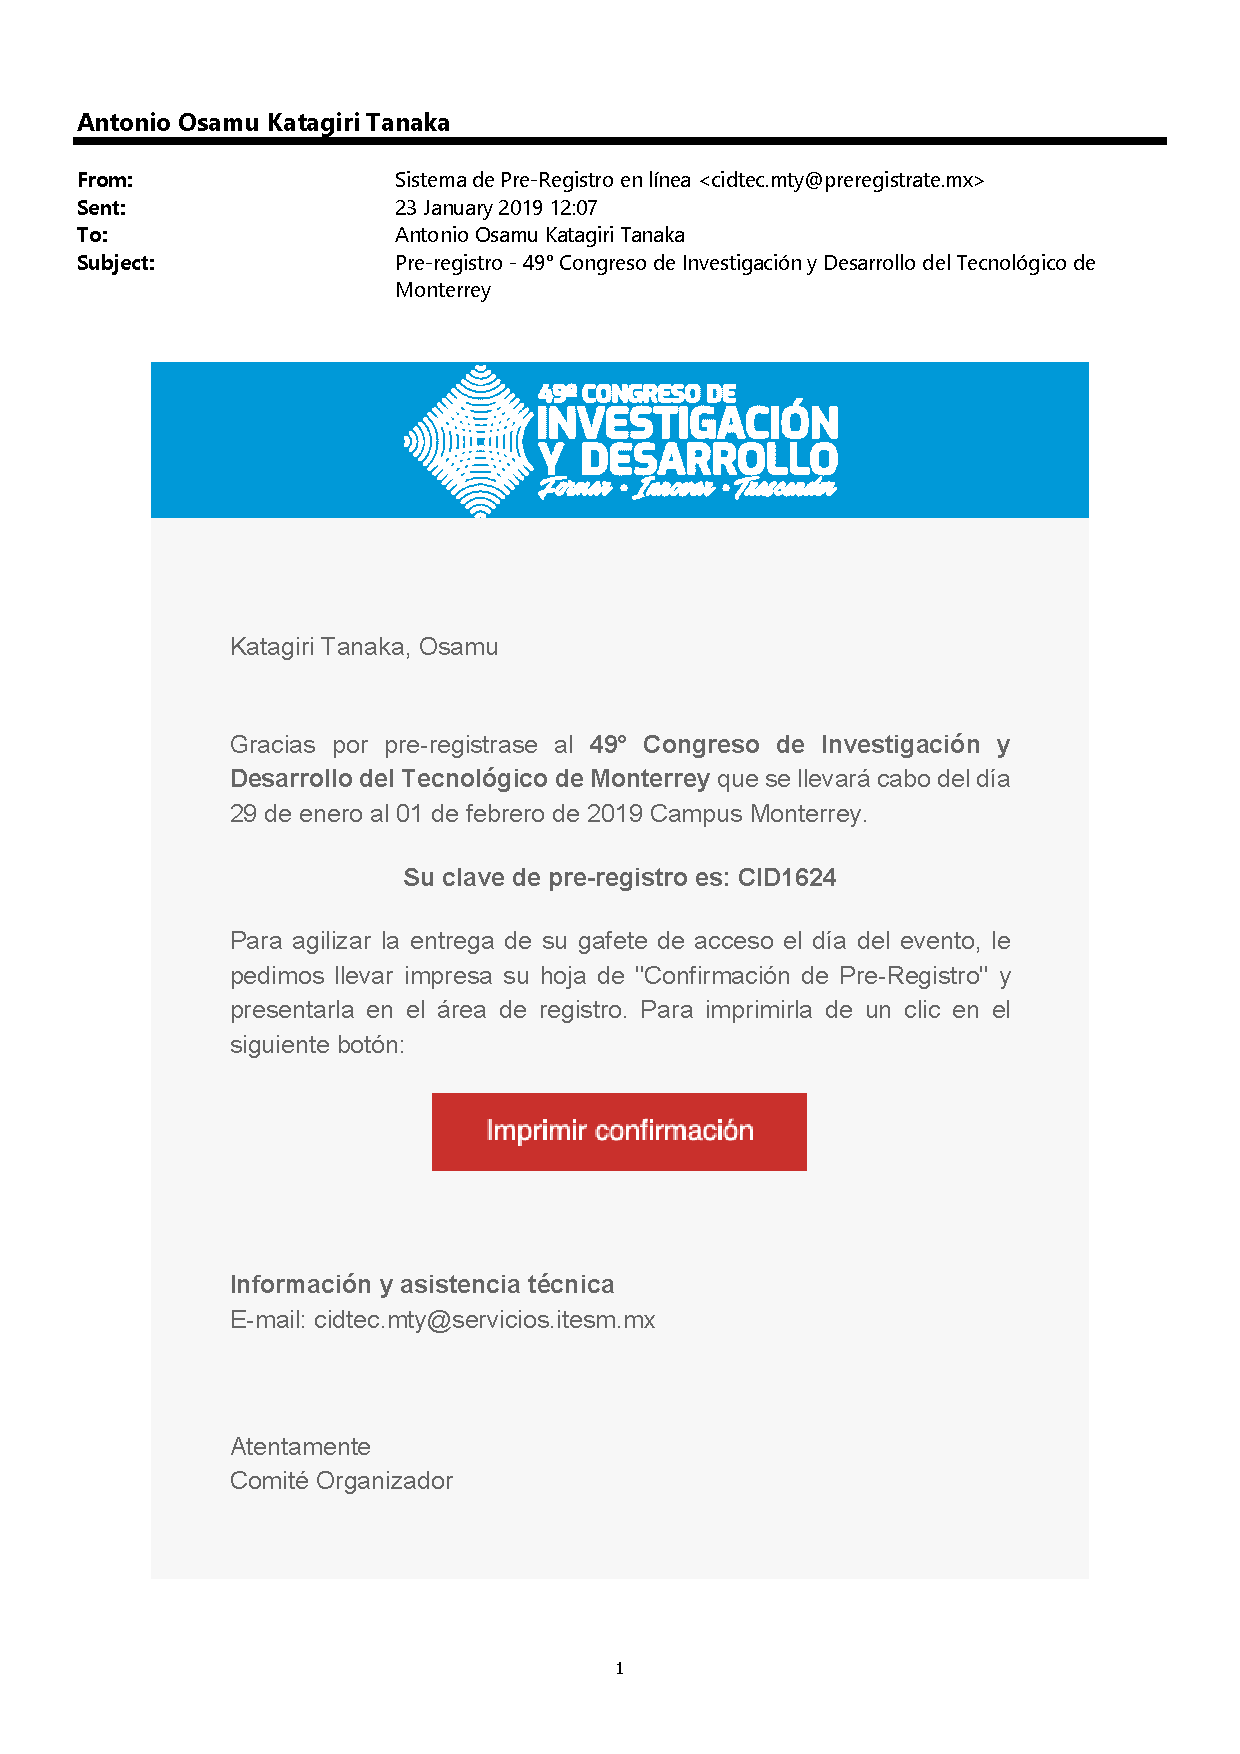
\includepdf[page=-]{pdf/49CIDTEC_preregistro}

%----------------------------------------------------------------------------------------%

\end{document}

%----------------------------------------------------------------------------------------%
